\documentclass[rnd]{mas_proposal}
% \documentclass[thesis]{mas_proposal}

\usepackage[utf8]{inputenc}
\usepackage{amsmath}
\usepackage{amsfonts}
\usepackage{amssymb}
\usepackage{graphicx}

\title{Comparison of Keyframe Extraction Techniques for Video Classification/Anomaly Detection}
\author{Rashid Ahamed Meeran Tajdeen}
\supervisors{(first supervisor)\\Santosh Thoduka (h-brs)}
\date{Sep 2023}

% \thirdpartylogo{path/to/your/image}

\begin{document}

\maketitle

\pagestyle{plain}

\section{Introduction}
    
Video is an integral part of our everyday lives, and is the most powerful form of multimedia. But storing, retrieving, indexing and summarizing videos have become very difficult. To resolve these problems key frame extraction technique is mainly used. In general, to minimize redundancy the key frame should be representative of the video content \cite{Sadiq2020}. A video can be more than one keyframes. Key frame extraction method speeds up the framework by choosing fundamental frames and thereby removing additional computation on redundant frames. Key frame extraction significantly reduces the video processing overhead time and increase the throughput \cite{Ragavan2020}. This project aims on comparing the different types of key frame extraction methods.

\subsection{Video Hierarchy}

Video has a complex structure that includes scene, shot, and frame \cite{Ragavan2020}.

\quad \textbf{Video:} A video is a series of scenes.

\quad \textbf{Scene:} A scene is a logical collection of shots.

\quad \textbf{Shot:} A shot is a series of frames in one continuous movement.

\quad \textbf{Frames:} A frame is nothing but an image.
\\
Key frames are the frames which can represent the salient content and information of the shot. Throughout this project, we consider video data with a single shot to reduce complexity.

\subsection{Video Abstraction Breakdown}

Video abstraction is a two step process as shown in Figure \ref{fig:video_abstraction}.

\begin{figure}[h!]
    \centering
    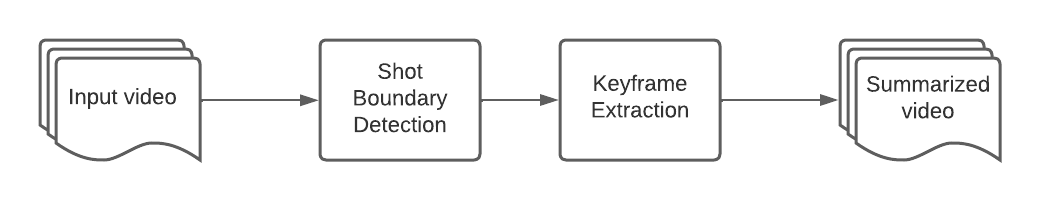
\includegraphics[width=\textwidth]{images/video_abstraction.png}
    \caption{Basic block diagram of video abstraction \cite{Sadiq2020}}
    \label{fig:video_abstraction}
\end{figure}

A video is generally comprised of one or more shots. So the first step would be to detect the boundaries and separate the video into different shots. Then keyframes are extracted from each shot separately.

\subsubsection{Shot Boundary Detection}

Shot boundary detection basically detects any transition in the video between 2 shots. Transition can be of two types which are the abrupt transitions and the gradual transitions. Abrupt transition is a sudden change of frames from one shot to another. Whereas gradual transition refers to when two shots are combined using some editing process such as fade-in, fade-out, dissolve, etc.

Throughout this work, we use a video dataset with single shots. This leads us to omit the shot boundary detection step completely thereby reducing the complexity.

\subsubsection{Keyframe Detection}

Keyframe extraction is an efficient method used to clearly express the important contents of a video file by extracting a set of representative frames and discarding the duplicated ones from the original video. These extracted keyframes are expected to represent and provide comprehensive visual information of the whole video.

\subsection{Shortcomings of Video Abstraction}

The demerits of various existing techniques in the area of keyframe extraction are as follows:

\begin{itemize}
    \item High computational time in the process of extracting the keyframes.
    \item Difficulty in extracting keyframes if the video contains
    \begin{itemize}
        \item Gradual transitioned frames (which causes interlooping of frames)
        \item Camera motions (such as panning, tilting or zooming)
        \item Sudden illumination (which might have made the camera sensor miss certain information)
    \end{itemize}
\end{itemize}

\subsection{Goal of this RnD}
    
The goal of this RnD is to improve the classification efficiency on a sewage pipe video dataset. In this process we compare the available methods to extract keyframes from the video shot. These keyframes, which are the representation of the video can replace the video itself as a dataset thereby reducing the complexity of both training and validation of a deep learning model.

\section{Problem Statement}

Video is an audiovisual data that comprises of large number of frames. Analyzing and processing such large amount of data is difficult to many applications. Even with deep learning, huge datasets would lead to large training times, high complexity and significantly increase the model size.

To overcome this we would have to do some pre-processing to the data. This can include image fine-tuning on frames, cropping frames \cite{Gharahbagh2022}, reducing the size of the data by reducing video resolution or by removing useless frames. Depending on the dataset, reducing video resolution is often costly to deal with as we might lose useful information from every frame.

There are lots of ways to dodge this problem and this works aims on implementing and comparing those by answering the the following research questions.

\textbf{Research Questions:}

\begin{itemize}
    \setlength{\itemindent}{3em}
    \item[\textbf{RQ1}] What are the state-of-the-art keyframe extraction methods?
    \item[\textbf{RQ2}] How efficient is a video classification model that selects random frames for training and validation?
    \item[\textbf{RQ3}] How does the methods from RQ1 affect the efficiency of the model in RQ2?
    \item[\textbf{RQ4}] What are the effects of introducing a pre-processing step (such as cropping frames) after the frame selection?
\end{itemize}

\section{Targeted Dataset}

For this project, we make use of the QV-Pipe dataset \cite{Liu2022}. This dataset consists of 9.6k videos, which are collected from real-world urban pipes. The total duration of all videos exceeds 55 hours. On average, each video has the duration of 20.7 seconds. Moreover, there are 1 normal class and 16 defect classes. Each video is annotated with multiple labels. Each video is comprised of single continuous shot.

\section{Evaluation Strategy}

As there is no specific way to say if the selected frames are the summary of a video, we compare the validation efficiency of different frame extraction methods to that of the random frame selection model.

\section{Related Work}

(TODO: ADD RELATED WORK)

\begin{tabular}{ |p{0.3cm}|p{4.2cm}|p{3cm}|p{2.5cm}|p{2.5cm}|  }
\hline
 & \textbf{Article} & \textbf{Method Used} & \textbf{Merits} & \textbf{Demerits} \\
\hline
\hline
1 &
Key Frame Extraction Based on Improved Hierarchical Clustering Algorithm &
K-means hierarchical Clustering algorithm &
Precision Ratio and recall Ratio is above 85\% &
Calculation of entropy is expensive \\

\hline
2 &
Key frame extraction using color histogram method &
Color histogram and edge detection method &
Less computational complexity and compression ratio is 98\% &
Absence of threshold conditions \\

\hline
3 &
An Algorithm for Shot Boundary Detection and Key Frame Extraction Using Histogram Difference &
Based on square histogram model &
Efficiency is about 95\% to 98\% &
Suitable only for “.avi” type \\

\hline
4 &
Key frame extraction based on entropy difference and perceptual hash &
Based on entropy difference and perceptual hash &
High accuracy and low miss rate &
Redundancy for background moving videos \\

\hline
5 &
A Dynamic Frame Selection Framework for Fast Video Recognition &
Adaframe: Memory-Augmented LSTM &
Low computational cost,  &
Enormous search space \\

\hline
6 &
The comparison and analysis of extracting video key frame &
Frame average; Histogram Averaging; Visual Content Matching &
 &
 \\

\hline
\end{tabular}

\section{Project Plan}

\subsection{Work Packages}
The bare minimum will include the following packages:
\begin{enumerate}
    \item[WP1] Literature review on the existing keyframe extraction techniques
    \begin{itemize}
        \item[T1.1] Understanding the importance of frame selection in video classification/anomaly detection.
        \item[T1.2] Literature search on the available methods for key-frame extraction.
        \item[T1.3] Identify and analyse the state-of-the-art methods that corresponds to our application.
    \end{itemize}
    \item[WP2] Experimental setup
    \begin{itemize}
        \item[T2.1] Implement a deep learning method with random frame selection to classify the chosen dataset.
        \item[T2.2] Introduce different key frame extraction methods.
        \item[T2.3] Introduce pre-processing steps (such as frame cropping) after frame extraction.
    \end{itemize}
    \item[WP3] Mid-term Report
    \begin{itemize}
        \item[T3.1] Submission of the mid-term report.
    \end{itemize}
    \item[WP4] Experimental analysis
    \begin{itemize}
        \item[T4.1] Compute efficiency of the basic deep learning model set up in T2.1 and have this as a reference measure.
        \item[T4.2] Compute efficiency of the deep learning model with other frame selection methods introduced in T2.2 separately and compare with the reference.
        \item[T4.3] Analyse the effect of introducing pre-processing steps by comparing the efficiency with the reference measure.
    \end{itemize}
    \item[WP5] Final Report
    \begin{itemize}
        \item[T5.1] Draft revision.
        \item[T5.2] Submission of the Final report.
    \end{itemize}
    
\end{enumerate}

\subsection{Milestones}
\begin{enumerate}
    \item[M1] Literature search
    \item[M2] Experimental setup
    \item[M3] Mid-term Report submission
    \item[M4] Experimental Analysis
    \item[M5] Final Report submission
\end{enumerate}

\subsection{Project Schedule}
    
(TODO: GANTT CHART)

\subsection{Deliverables}

\subsubsection*{Minimum Viable}
\begin{itemize}
    \item State of the art analysis.
    \item 
\end{itemize}

\subsubsection*{Expected}
\begin{itemize}
    \item 
\end{itemize}

\subsubsection*{Desired}
\begin{itemize}
    \item 
\end{itemize}


\nocite{*}

\bibliographystyle{unsrt} % Use the plainnat bibliography style
\bibliography{bibliography.bib} % Use the bibliography.bib file as the source of references


\end{document}
